% fig_memory.tex - Dual-layer experiential memory (standalone -> PDF)
\documentclass[tikz,border=6pt]{standalone}
\usepackage{tikz}
\usetikzlibrary{arrows.meta,positioning,fit,backgrounds,calc,shapes.geometric}
\definecolor{ours}{HTML}{C0392B}
\definecolor{slate}{HTML}{2C3E50}
\definecolor{teal}{HTML}{16A085}
\definecolor{purp}{HTML}{8E44AD}
\definecolor{blue}{HTML}{2980B9}
\definecolor{lg}{HTML}{ECF0F1}
\definecolor{mgd}{HTML}{7F8C8D}
\begin{document}
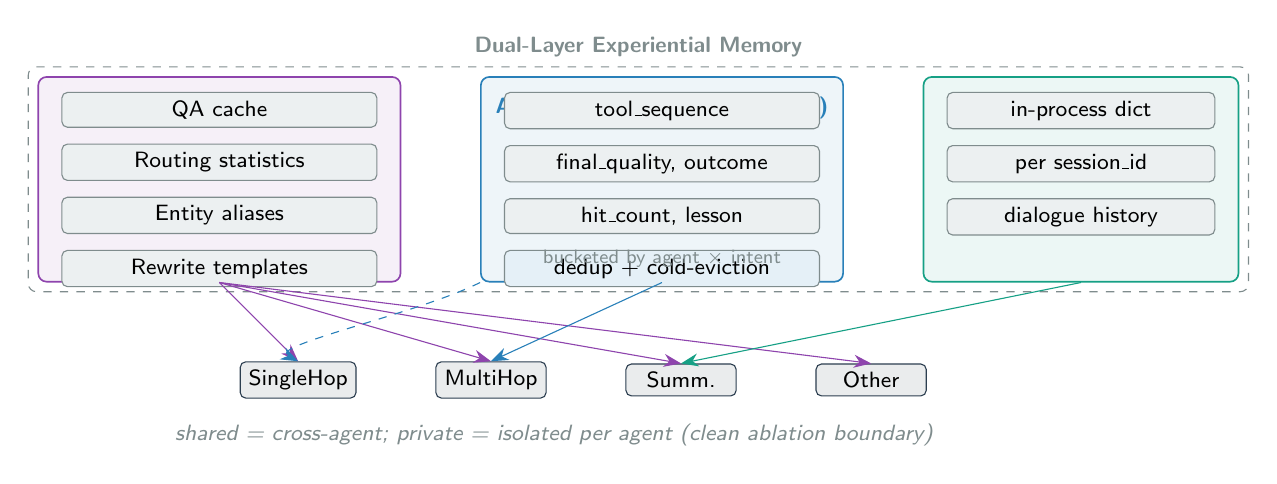
\begin{tikzpicture}[
  font=\small\sffamily,
  >={Stealth[length=2.2mm]},
  node distance=5mm and 10mm,
  col/.style={draw=slate, rounded corners=3pt, align=center, inner sep=5pt,
              minimum width=46mm, minimum height=26mm, fill=white, line width=0.6pt},
  item/.style={draw=mgd, rounded corners=2pt, align=center, inner sep=3pt,
               fill=lg, minimum width=40mm, line width=0.4pt, font=\footnotesize\sffamily},
  hd/.style={font=\footnotesize\sffamily\bfseries},
  agent/.style={draw=slate, fill=slate!10, rounded corners=2pt, inner sep=3pt,
                minimum width=14mm, font=\footnotesize\sffamily},
]
% --- Shared memory column ---
\node[col, fill=purp!8, draw=purp] (sh) {};
\node[hd, color=purp] at ($(sh.north)+(0,-4mm)$) {Shared Memory (JSON)};
\node[item, below=2mm of sh.north] (qa) {QA cache};
\node[item, below=2mm of qa] (rs) {Routing statistics};
\node[item, below=2mm of rs] (ea) {Entity aliases};
\node[item, below=2mm of ea] (rt) {Rewrite templates};

% --- Private memory column ---
\node[col, right=of sh, fill=blue!8, draw=blue] (pr) {};
\node[hd, color=blue] at ($(pr.north)+(0,-4mm)$) {Agent Private Memory (JSONL)};
\node[item, below=2mm of pr.north] (t1) {tool\_sequence};
\node[item, below=2mm of t1] (t2) {final\_quality, outcome};
\node[item, below=2mm of t2] (t3) {hit\_count, lesson};
\node[item, below=2mm of t3, fill=blue!12] (t4) {dedup + cold-eviction};
\node[font=\scriptsize\sffamily, color=mgd] at ($(pr.south)+(0,3mm)$)
  {bucketed by agent $\times$ intent};

% --- Session memory column ---
\node[col, right=of pr, fill=teal!8, draw=teal, minimum width=40mm] (se) {};
\node[hd, color=teal] at ($(se.north)+(0,-4mm)$) {Session Memory};
\node[item, below=2mm of se.north, minimum width=34mm] (s1) {in-process dict};
\node[item, below=2mm of s1, minimum width=34mm] (s2) {per session\_id};
\node[item, below=2mm of s2, minimum width=34mm] (s3) {dialogue history};

% --- agents row (consumers) ---
\node[agent, below=10mm of sh.south, xshift=10mm] (a1) {SingleHop};
\node[agent, right=of a1] (a2) {MultiHop};
\node[agent, right=of a2] (a3) {Summ.};
\node[agent, right=of a3] (a4) {Other};

% shared: cross-agent read (all agents)
\foreach \a in {a1,a2,a3,a4} \draw[->, purp] (sh.south) -- (\a.north);
% private: isolated (only MultiHop shown reading its own, dashed for others)
\draw[->, blue] (pr.south) -- (a2.north);
\draw[->, blue, dashed] (pr.south west) ..controls +(-8mm,-4mm) and +(-4mm,2mm).. (a1.north);
% session
\draw[->, teal] (se.south) -- (a3.north);

\node[font=\footnotesize\sffamily\itshape, color=mgd, below=2mm of a2.south, xshift=8mm]
  {shared = cross-agent;  private = isolated per agent (clean ablation boundary)};

\begin{scope}[on background layer]
  \node[draw=mgd, dashed, rounded corners=3pt, fit=(sh)(pr)(se),
        label={[font=\footnotesize\sffamily\bfseries,color=mgd]above:Dual-Layer Experiential Memory}] {};
\end{scope}
\end{tikzpicture}
\end{document}
